%%%%%%%%%%%%%%%%%%%%%%%%%%%%%%%%%%%%%%%%%%%%%%%%%%%%%%%%%%%%%%%%%%%%%%%%%%%%%%%%%%
\begin{frame}[fragile]\frametitle{}
\begin{center}
{\Large Niyama नियम}
\end{center}
\end{frame}


%%%%%%%%%%%%%%%%%%%%%%%%%%%%%%%%%%%%%%%%%%%%%%%%%%%%%%%%%%%
\begin{frame}[fragile]\frametitle{Introduction}

Shaucha santosha tapah swadhyayeshwara pranidhanani niyamah

शौच-संतोष-तप:-स्वाध्यायेश्वरप्रणिधानानि नियमा:||

	\begin{itemize}
	\item The  collective  disciplines  of 
Niyama  are  Physical  \&  mental 
purity, contentment, austerity,
self  study  of  holy  books  and 
scriptures and devotion to god. 
\item One  must  dedicate  the  fruits 
and one’s action to god.
	\end{itemize}

\end{frame}

%%%%%%%%%%%%%%%%%%%%%%%%%%%%%%%%%%%%%%%%%%%%%%%%%%%%%%%%%%%
\begin{frame}[fragile]\frametitle{Ethical Foundations}

	\begin{itemize}
	\item Shaucha शौच : cleanliness or purity
	\item Santosha संतोष : contentment
	\item Tapas तप : fervour, discipline in sadhana
	\item Svadhyaya स्वाध्याय : study of scriptures/self
	\item Ishvara pranidhana ईश्वरप्रणिधान surrender to the cosmos/creator
	\end{itemize}

\end{frame}


%%%%%%%%%%%%%%%%%%%%%%%%%%%%%%%%%%%%%%%%%%%%%%%%%%%%%%%%%%%
\begin{frame}[fragile]\frametitle{Shaucha शौच Purity }
   \begin{columns}
    \begin{column}[t]{0.7\linewidth}
	
	\begin{itemize}
	\item Cleanliness
	\item Cleansing of  inner and an outer aspects
	\item Cleansing the exterior: physical exercises or techniques of purification 
	\item Cleansing the interior: clearing the mind of disturbing emotions like hatred, passion, anger, lust, greed, delusion and pride.

	\end{itemize}
	    \end{column}
    \begin{column}[t]{0.3\linewidth}
\begin{center}
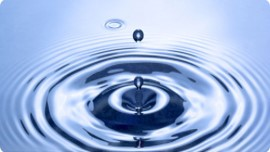
\includegraphics[width=0.8\linewidth,keepaspectratio]{yog31}

\end{center}
    \end{column}
  \end{columns}
  
  \tiny{(Ref: Yoga: The art of happiness - Yoga Integral Esoterique)}

\end{frame}


%%%%%%%%%%%%%%%%%%%%%%%%%%%%%%%%%%%%%%%%%%%%%%%%%%%%%%%%%%%
\begin{frame}[fragile]\frametitle{Santosha संतोष  Contentment}
   \begin{columns}
    \begin{column}[t]{0.7\linewidth}
	
	\begin{itemize}
	\item Modesty; being content with what we have
	\item Acceptance of events we face, but preparing to transform what we can transform
	\item Experiencing life’s difficulties - we have the opportunity to grow 
	\item Understanding that there is a purpose for everything, even if the whole picture is not revealed to us 
	\item Being happy with what we have, rather than unhappy about what we don't have
	\item Contentment is a inner quality not dependent on exterior circumstances 

	\end{itemize}
	    \end{column}
    \begin{column}[t]{0.3\linewidth}
\begin{center}

\includegraphics[width=0.8\linewidth,keepaspectratio]{yog32}

\end{center}
    \end{column}
  \end{columns}
  
  \tiny{(Ref: Yoga: The art of happiness - Yoga Integral Esoterique)}

\end{frame}


%%%%%%%%%%%%%%%%%%%%%%%%%%%%%%%%%%%%%%%%%%%%%%%%%%%%%%%%%%%
\begin{frame}[fragile]\frametitle{Tapas तप   Disciplined Efforts}
   \begin{columns}
    \begin{column}[t]{0.7\linewidth}
	
	\begin{itemize}
	\item Disciplined use of our energy 
	\item Literally to heat, put on a flame, being burned
	\item The conscious effort to accomplish a spiritual goal (ultimate goal is fusion with the Superior Consciousness) and burn up all the inferior desires that stand in our way
	\item This effort implies our transformation through the practice of the stages of yoga: following yama and nyiama, postures, pranayama, meditation, etc.
	\item Such efforts must be done whether the exterior conditions are good or not
	\end{itemize}
	    \end{column}
    \begin{column}[t]{0.3\linewidth}
\begin{center}

\includegraphics[width=0.8\linewidth,keepaspectratio]{yog33}

\end{center}
    \end{column}
  \end{columns}
  
  \tiny{(Ref: Yoga: The art of happiness - Yoga Integral Esoterique)}

\end{frame}

%%%%%%%%%%%%%%%%%%%%%%%%%%%%%%%%%%%%%%%%%%%%%%%%%%%%%%%%%%%
\begin{frame}[fragile]\frametitle{Svadhyaya स्वाध्याय   Self-study}
   \begin{columns}
    \begin{column}[t]{0.7\linewidth}
	
	\begin{itemize}
	\item Sva = Self; adhyaya = examination/study
	\item ``Education for self-revelation'' 
	\item The study of sacred texts that give us reflections about the Self : Yoga-Sutra, Bhagavat-Gita, Siva Samhita, Hatha Yoga Pradipika, the Bible, the Koran, etc.
	\item Any activity that cultivates self-reflective consciousness  and self-awareness 
	\item ``Know yourself and you will know the entire  universe''

	\end{itemize}
	    \end{column}
    \begin{column}[t]{0.3\linewidth}
\begin{center}

\includegraphics[width=0.8\linewidth,keepaspectratio]{yog34}

\end{center}
    \end{column}
  \end{columns}
  
  \tiny{(Ref: Yoga: The art of happiness - Yoga Integral Esoterique)}

\end{frame}

%%%%%%%%%%%%%%%%%%%%%%%%%%%%%%%%%%%%%%%%%%%%%%%%%%%%%%%%%%%
\begin{frame}[fragile]\frametitle{Ishvara pranidhana ईश्वरप्रणिधान Celebration of the Supreme Consciousness }
   \begin{columns}
    \begin{column}[t]{0.7\linewidth}
	
	\begin{itemize}
	\item Ishvara = last degree in a hierarchy, God, Superior Self Atman, Supreme Consciousness 
	\item Pranidhana = continuous devotion
	\item To make a continuous effort to reach the state of Supreme Consciousness 
	\item The contemplation of Isvara/ Supreme Consciousness in order to become attuned to it.


	\end{itemize}
	    \end{column}
    \begin{column}[t]{0.3\linewidth}
\begin{center}

\includegraphics[width=0.8\linewidth,keepaspectratio]{yog35}

\end{center}
    \end{column}
  \end{columns}
  
  \tiny{(Ref: Yoga: The art of happiness - Yoga Integral Esoterique)}

\end{frame}


%%%%%%%%%%%%%%%%%%%%%%%%%%%%%%%%%%%%%%%%%%%%%%%%%%%%%%%%%%%
\begin{frame}[fragile]\frametitle{Summary}

\begin{center}
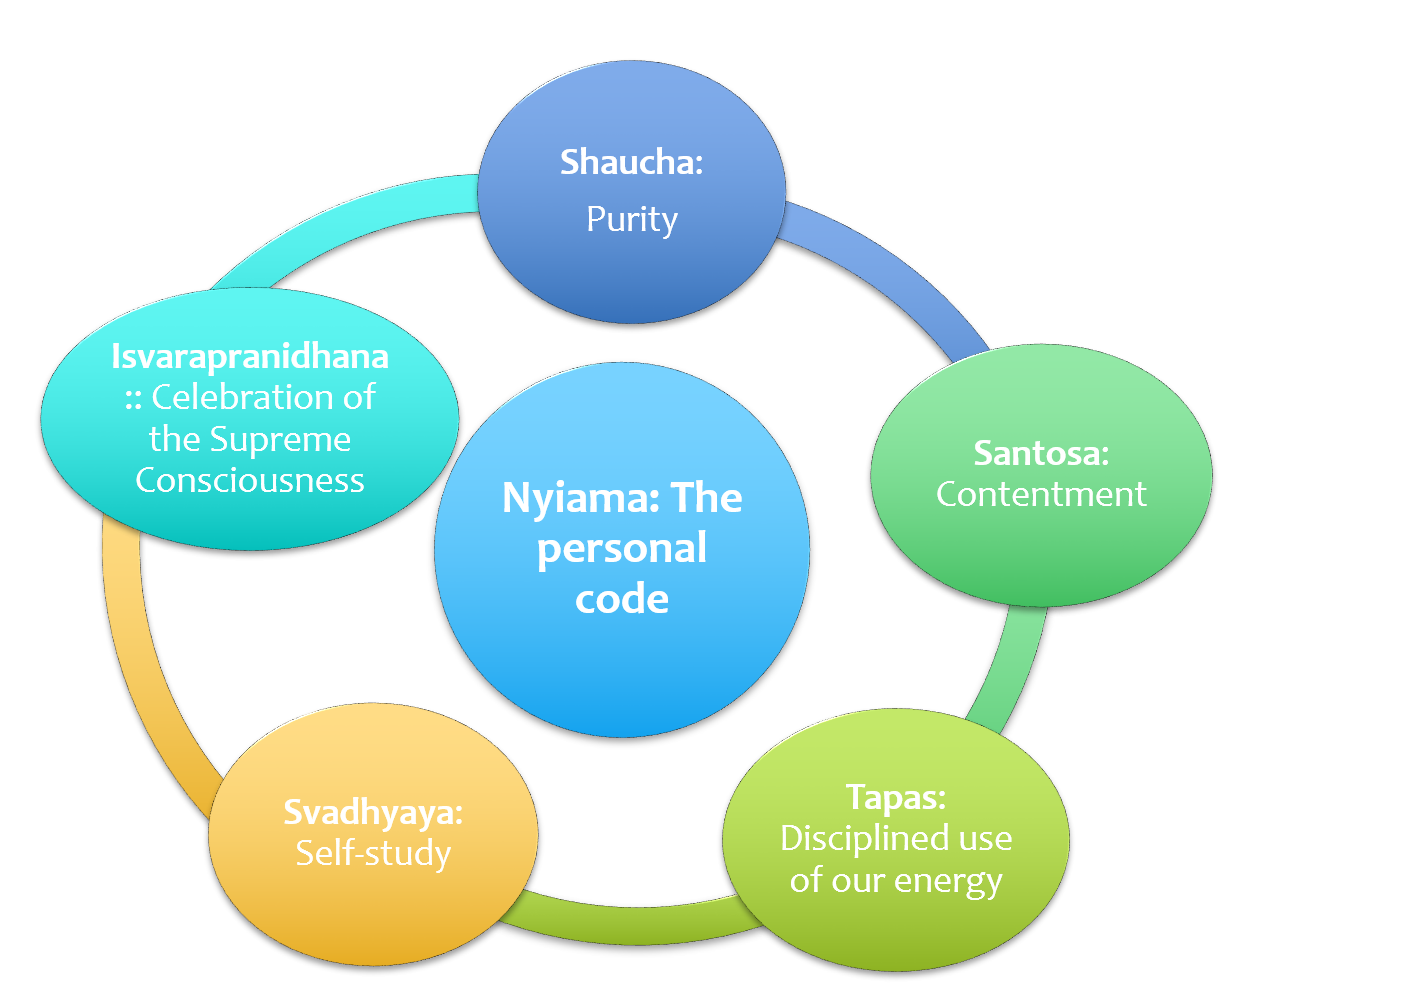
\includegraphics[width=0.8\linewidth,keepaspectratio]{yog30}

\end{center}

  
  \tiny{(Ref: Yoga: The art of happiness - Yoga Integral Esoterique)}

\end{frame}